%==============================================================================
% TCC defense slides, Inf beamer theme (Instituto de Informatica, UFRGS)
%
% 20 minutes, about one minute per content slide. Background and related work
% stay minimal: the context needed to follow the work goes in the Introduction.
%==============================================================================
\documentclass[aspectratio=169]{beamer}

\usepackage[T1]{fontenc}
\usepackage[utf8]{inputenc}
\usepackage[english]{babel}
\usepackage{graphicx}
\usepackage{amssymb}
\usepackage{pifont}
\usepackage{tikz}
\usetikzlibrary{positioning,arrows.meta,calc}

\usetheme{Inf}

\graphicspath{{figures/}}

% Frame colors of the PON diagram, the same as the thesis figure
\definecolor{PktA}{RGB}{166,206,227}
\definecolor{PktB}{RGB}{178,223,138}
\definecolor{PktC}{RGB}{253,191,111}

% The tier ladder drawn with confidence alone (false) or with WattLadder (true)
\newif\ifLadderEnergy

% Gray note marking what a slide will hold, removed as each slide is written
\newcommand{\placeholder}[1]{{\color{InfGray}\itshape #1}}

% The one sentence a slide should leave with the audience
\newcommand{\takeaway}[1]{\par\vfill{\centering\large #1\par}}

% Source line for a borrowed figure or claim
\newcommand{\source}[1]{{\par\raggedleft\tiny\color{InfGray}#1\par}}

% A large figure with a short caption and its source
\newcommand{\stat}[3]{%
  \centering
  {\fontsize{34}{38}\selectfont\bfseries\color{InfRed}#1}\par\medskip
  {\small #2}\par\smallskip
  {\tiny\color{InfGray}#3}\par}

\newcommand{\yes}{{\color{InfBlack}\checkmark}}
\newcommand{\no}{{\color{InfLightGray}\ding{55}}}

%------------------------------------------------------------------------------
% Title page
%------------------------------------------------------------------------------
\title[WattLadder]
      {WattLadder: Energy-Aware Recursive Offloading for LLM Inference over
       Passive Optical Networks}

\subtitle{Advisor: Prof.~Dr.~Gabriel Luca Nazar\\
          Co-advisor: Prof.~Dr.~Dennis Giovani Balreira}

\date{2026}

\author{Diego Hommerding Amorim}
\institute{Instituto de Informática --- UFRGS}

\begin{document}

\InfTitlePage

\begin{frame}
  \frametitle{Outline}
  \tableofcontents
\end{frame}

%------------------------------------------------------------------------------
\section{Introduction}
% About 5 minutes: why energy, the tiers, the PON, the gap and the proposal
%------------------------------------------------------------------------------

\begin{frame}
  \frametitle{Why Energy}
  \begin{columns}[t]
    \begin{column}{0.45\textwidth}
      \stat{$\approx$40\%}{of US adults aged 18--64 used generative AI in 2024}
        {Bick, Blandin and Deming, 2026}
    \end{column}
    \begin{column}{0.45\textwidth}
      \stat{0.24 Wh}{per median Gemini text prompt, about 860~J, counted over
        the whole data center}{Elsworth et al., 2025}
    \end{column}
  \end{columns}
  \takeaway{Small for one prompt, but paid again on every query, so the energy
    of inference grows with its use.}
\end{frame}

\begin{frame}
  \frametitle{Tiered LLM Inference}
  \begin{columns}[c]
    \begin{column}{0.66\textwidth}
      \centering
      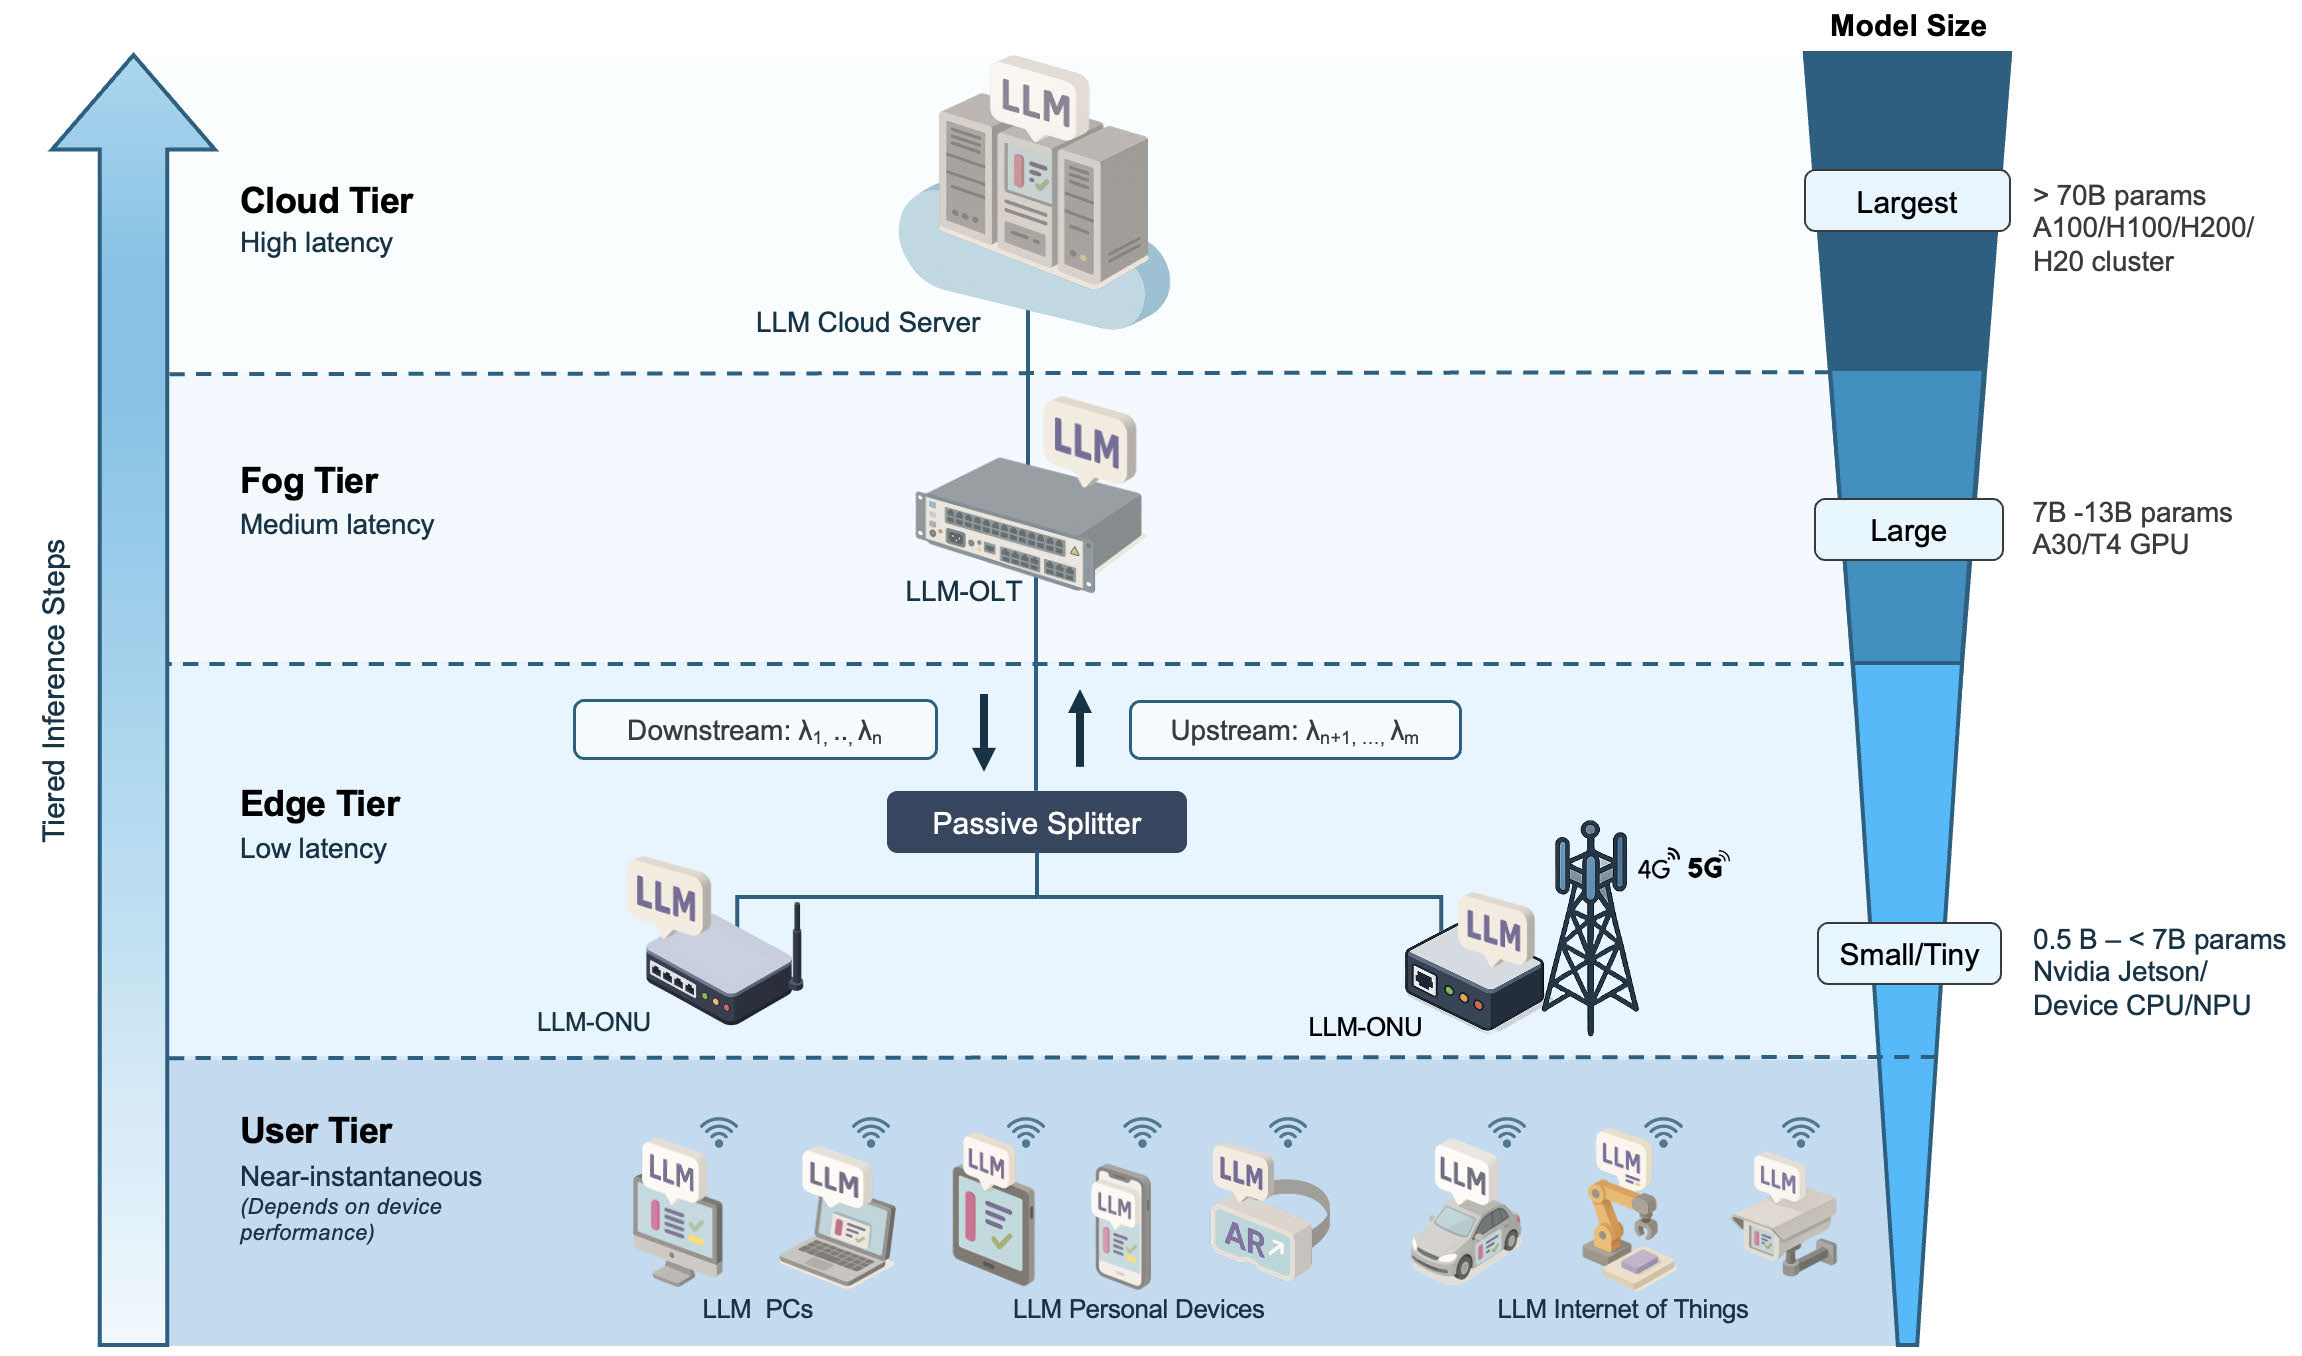
\includegraphics[width=\textwidth,height=0.56\textheight,keepaspectratio]{pakpahan2026_fig1_tiered_continuum}
      \source{Pakpahan and Hwang, 2026}
    \end{column}
    \begin{column}{0.30\textwidth}
      \stat{98\%}{lower cost at GPT-4's quality with a model cascade}
        {Chen, Zaharia and Zou, 2024}
    \end{column}
  \end{columns}
  \takeaway{Each tier runs a larger model than the one below, and a query
    climbs until a tier is confident in its answer.}
\end{frame}

\begin{frame}
  \frametitle{The Access Network}
  \centering
  % PON tree with the downstream broadcast, simplified from the thesis figure
\begin{tikzpicture}[
    font=\footnotesize,
    box/.style={draw, thick, rounded corners=2pt, minimum width=1.3cm,
                minimum height=0.7cm, fill=white},
    home/.style={draw, rounded corners=2pt, minimum width=1.1cm,
                 minimum height=0.55cm, fill=black!5, font=\scriptsize},
    split/.style={draw, thick, circle, minimum size=0.45cm, inner sep=0pt,
                  fill=white},
    fiber/.style={thick},
    pkt/.style={draw, rounded corners=1pt, minimum size=0.34cm, inner sep=0pt,
                font=\tiny\bfseries},
    p1/.style={pkt, fill=PktA}, p2/.style={pkt, fill=PktB}, p3/.style={pkt, fill=PktC},
    note/.style={font=\scriptsize, text=InfGray}
  ]
  \node[box] (olt) at (0,0) {OLT};
  \node[note, below=3pt of olt] {central office};
  \node[split] (sp) at (3.4,0) {};
  \node[note, below=3pt of sp] {splitter};
  \draw[fiber] (olt) -- (sp);
  \foreach \k/\x in {3/1.2, 2/1.7, 1/2.2} { \node[p\k] at (\x,0) {\k}; }
  \foreach \i/\y in {1/1.4, 2/0, 3/-1.4} {
    \node[box] (onu\i) at (7.4,\y) {ONU \i};
    \node[home] (usr\i) at (9.9,\y) {home \i};
    \draw[fiber] (sp) -- (onu\i.west);
    \draw[fiber] (onu\i.east) -- (usr\i.west);
    % every branch carries every frame, the ONU keeps only its own
    \foreach \k/\t in {3/0.45, 2/0.6, 1/0.75} {
      \node[p\k] at ($(sp)!\t!(onu\i.west)$) {\k};
    }
    \node[p\i] at ($(onu\i.east)!0.5!(usr\i.west)$) {\i};
  }
  \node[note] at (8.65,-2.1) {\ldots\ thousands of homes per OLT};
\end{tikzpicture}

  \takeaway{One OLT serves thousands of homes, and every frame it sends
    downstream reaches all of them.}
\end{frame}

\begin{frame}
  \frametitle{The Gap}
  \LadderEnergyfalse
  \begin{columns}[c]
    \begin{column}{0.42\textwidth}
      \centering
      % The three tiers of the case study. \LadderEnergy switches the escalation
% labels from confidence alone to WattLadder's and adds the skip arrow.
% \LadderModels names each tier's model and accuracy (the case study);
% without it the tiers say only small, medium and large model (the
% introduction). \LadderHardware names each tier's device in gray at its
% right, and \LadderLabels (on by default) labels the escalation arrows.
% Outer labels have no inner sep, so the picture's box ends at its ink.
\begin{tikzpicture}[
    font=\footnotesize,
    tier/.style={draw, thick, rounded corners=3pt, minimum width=3.3cm,
                 minimum height=0.8cm, fill=white, align=center},
    escalate/.style={-{Stealth[length=2mm]}, thick},
    answerline/.style={-{Stealth[length=2mm]}, thick, InfGray},
    lbl/.style={font=\scriptsize, align=right, inner sep=0pt, xshift=-5.33pt}
  ]
  \ifLadderModels
    \def\oltmodel{Qwen2.5-7B \,\textperiodcentered\, 91.7\%}%
    \def\onumodel{Qwen2.5-1.5B \,\textperiodcentered\, 68.8\%}%
    \def\usrmodel{Llama-3.2-1B \,\textperiodcentered\, 47.2\%}%
  \else
    \def\oltmodel{large model}%
    \def\onumodel{medium model}%
    \def\usrmodel{small model}%
  \fi
  \node[tier] (olt) at (0,3.1) {\textbf{OLT}\\[-2pt]{\scriptsize\oltmodel}};
  \node[tier] (onu) at (0,1.55) {\textbf{ONU}\\[-2pt]{\scriptsize\onumodel}};
  \node[tier] (usr) at (0,0) {\textbf{Phone}\\[-2pt]{\scriptsize\usrmodel}};

  \draw[escalate] (0,-0.85) node[below=3.33pt, inner sep=0pt, font=\scriptsize] {query} -- (usr);
  \ifLadderEnergy
    \draw[escalate, InfRed] (usr) -- node[lbl, left, text=InfRed] {confidence\\+ energy} (onu);
    \draw[escalate, InfRed] (onu) -- node[lbl, left, text=InfRed] {confidence\\+ energy} (olt);
    \draw[escalate, InfRed, dashed] (usr.west) to[out=150, in=210]
      node[lbl, left, text=InfRed, pos=0.5, xshift=-2pt] {skip\\the ONU} (olt.west);
  \else
    \ifLadderLabels
      \draw[escalate] (usr) -- node[lbl, left] {not confident} (onu);
      \draw[escalate] (onu) -- node[lbl, left] {not confident} (olt);
    \else
      \draw[escalate] (usr) -- (onu);
      \draw[escalate] (onu) -- (olt);
    \fi
  \fi
  \ifLadderAnswers
    \foreach \t in {usr, onu, olt} {
      \draw[answerline] (\t.east) -- ++(0.45,0)
        node[right=3.33pt, inner sep=0pt, font=\scriptsize, text=InfGray] {answer};
    }
  \fi
  \ifLadderHardware
    \foreach \t/\device in {usr/{OnePlus 15 phone},
                            onu/{Raspberry Pi 5\\with Hailo-10H},
                            olt/{server with\\one NVIDIA L4}} {
      \node[right=6pt, inner sep=0pt, font=\scriptsize, text=InfGray, align=left]
        at (\t.east) {\device};
    }
  \fi
\end{tikzpicture}

    \end{column}
    \begin{column}{0.54\textwidth}
      \centering
      {\small Energy one query adds}\par\medskip
      % Energy one query of the mean GSM8K lengths adds at each tier (thesis Table
% "Energy of the three tiers", marginal column, and the OLT's 840 J vs 5 J).
% Text labels have no inner sep, so the picture's box ends at its ink.
\begin{tikzpicture}[
    font=\footnotesize,
    bar/.style={minimum height=0.5cm, inner sep=0pt, anchor=west},
    tierlabel/.style={anchor=east, align=right, inner sep=0pt},
    value/.style={anchor=west, inner sep=0pt, font=\footnotesize\bfseries}
  ]
  \def\jscale{0.0036}  % cm per joule: 840 J fills about 3 cm
  \foreach \row/\tiername/\joules/\barcolor in {
      0/{Phone}/15.7/InfGray,
      1/{ONU}/92/InfGray,
      2/{OLT, idle}/840/InfRed,
      3/{OLT, batching}/5/InfRed} {
    \pgfmathsetmacro{\barlen}{max(\joules*\jscale, 0.06)}
    \node[tierlabel] at (-0.267, -\row*0.85) {\tiername};
    \node[bar, fill=\barcolor, minimum width=\barlen cm] at (0, -\row*0.85) {};
    \node[value, text=\barcolor] at (\barlen+0.217, -\row*0.85) {\joules~J};
  }
  \draw[thick] (0,0.4) -- (0,-2.95);
\end{tikzpicture}

    \end{column}
  \end{columns}
  \takeaway{Escalation looks only at confidence, while the cost of a query at
    the OLT swings from 840~J to 5~J with its load.}
\end{frame}

\begin{frame}
  \frametitle{This Work}
  \LadderEnergytrue
  \begin{columns}[c]
    \begin{column}{0.52\textwidth}
      \centering
      % The three tiers of the case study. \LadderEnergy switches the escalation
% labels from confidence alone to WattLadder's and adds the skip arrow.
% \LadderModels names each tier's model and accuracy (the case study);
% without it the tiers say only small, medium and large model (the
% introduction). \LadderHardware names each tier's device in gray at its
% right, and \LadderLabels (on by default) labels the escalation arrows.
% Outer labels have no inner sep, so the picture's box ends at its ink.
\begin{tikzpicture}[
    font=\footnotesize,
    tier/.style={draw, thick, rounded corners=3pt, minimum width=3.3cm,
                 minimum height=0.8cm, fill=white, align=center},
    escalate/.style={-{Stealth[length=2mm]}, thick},
    answerline/.style={-{Stealth[length=2mm]}, thick, InfGray},
    lbl/.style={font=\scriptsize, align=right, inner sep=0pt, xshift=-5.33pt}
  ]
  \ifLadderModels
    \def\oltmodel{Qwen2.5-7B \,\textperiodcentered\, 91.7\%}%
    \def\onumodel{Qwen2.5-1.5B \,\textperiodcentered\, 68.8\%}%
    \def\usrmodel{Llama-3.2-1B \,\textperiodcentered\, 47.2\%}%
  \else
    \def\oltmodel{large model}%
    \def\onumodel{medium model}%
    \def\usrmodel{small model}%
  \fi
  \node[tier] (olt) at (0,3.1) {\textbf{OLT}\\[-2pt]{\scriptsize\oltmodel}};
  \node[tier] (onu) at (0,1.55) {\textbf{ONU}\\[-2pt]{\scriptsize\onumodel}};
  \node[tier] (usr) at (0,0) {\textbf{Phone}\\[-2pt]{\scriptsize\usrmodel}};

  \draw[escalate] (0,-0.85) node[below=3.33pt, inner sep=0pt, font=\scriptsize] {query} -- (usr);
  \ifLadderEnergy
    \draw[escalate, InfRed] (usr) -- node[lbl, left, text=InfRed] {confidence\\+ energy} (onu);
    \draw[escalate, InfRed] (onu) -- node[lbl, left, text=InfRed] {confidence\\+ energy} (olt);
    \draw[escalate, InfRed, dashed] (usr.west) to[out=150, in=210]
      node[lbl, left, text=InfRed, pos=0.5, xshift=-2pt] {skip\\the ONU} (olt.west);
  \else
    \ifLadderLabels
      \draw[escalate] (usr) -- node[lbl, left] {not confident} (onu);
      \draw[escalate] (onu) -- node[lbl, left] {not confident} (olt);
    \else
      \draw[escalate] (usr) -- (onu);
      \draw[escalate] (onu) -- (olt);
    \fi
  \fi
  \ifLadderAnswers
    \foreach \t in {usr, onu, olt} {
      \draw[answerline] (\t.east) -- ++(0.45,0)
        node[right=3.33pt, inner sep=0pt, font=\scriptsize, text=InfGray] {answer};
    }
  \fi
  \ifLadderHardware
    \foreach \t/\device in {usr/{OnePlus 15 phone},
                            onu/{Raspberry Pi 5\\with Hailo-10H},
                            olt/{server with\\one NVIDIA L4}} {
      \node[right=6pt, inner sep=0pt, font=\scriptsize, text=InfGray, align=left]
        at (\t.east) {\device};
    }
  \fi
\end{tikzpicture}

    \end{column}
    \begin{column}{0.44\textwidth}
      \begin{enumerate}
        \setlength{\itemsep}{8pt}
        \item \textbf{WattLadder}
        \item \textbf{Energy model} of the tiers
        \item OLT's cost: \textbf{timetable} or \textbf{broadcast}
        \item \textbf{Simulation} at equal accuracy
      \end{enumerate}
    \end{column}
  \end{columns}
  \takeaway{Same accuracy as confidence alone, with about half the energy at
    20,000 households.}
\end{frame}

%------------------------------------------------------------------------------
\section{Related Work}
% About 1 minute: where this work stands, no paper-by-paper review
%------------------------------------------------------------------------------

\begin{frame}
  \frametitle{Positioning}
  \centering
  \small
  \renewcommand{\arraystretch}{1.3}
  \begin{tabular}{lccc}
    & \shortstack{Across\\network tiers} & \shortstack{Decides at\\every tier}
      & \shortstack{Weighs\\energy} \\
    \hline
    RecServe {\tiny\color{InfGray}(Wu et al., 2025)}             & \yes & \yes & \no  \\
    Tiered PON {\tiny\color{InfGray}(Pakpahan and Hwang, 2026)}   & \yes & \yes & \no  \\
    PerLLM {\tiny\color{InfGray}(Yang et al., 2024)}              & \yes & \no  & \yes \\
    CR$^2$ {\tiny\color{InfGray}(Xue et al., 2026)}               & \yes & \no  & \yes \\
    GreenServ {\tiny\color{InfGray}(Ziller et al., 2026)}         & \no  & \no  & \yes \\
    \hline
    {\color{InfRed}\textbf{WattLadder}}                           & \yes & \yes & {\color{InfRed}\checkmark} \\
  \end{tabular}
  \takeaway{Tiered works decide at every tier but ignore energy; energy-aware
    works decide once, before any model has answered.}
\end{frame}

%------------------------------------------------------------------------------
\section{Methodology}
% About 6 minutes: overview level, formulas by purpose, no derivations
%------------------------------------------------------------------------------

\begin{frame}
  \frametitle{Case Study}
  \placeholder{Three tiers: phone (Llama-3.2-1B, 47.2\%), ONU
    (Qwen2.5-1.5B, 68.8\%), OLT (Qwen2.5-7B, 91.7\%). GSM8K, recorded
    answers replayed}
\end{frame}

\begin{frame}
  \frametitle{WattLadder}
  \placeholder{The decision at each tier: run the query or send it up,
    then answer or escalate. Confidence test plus expected energy.
    Figure: beta\_knob}
\end{frame}

\begin{frame}
  \frametitle{Learning the OLT's Cost}
  \placeholder{Timetable learned in advance vs. cost report broadcast on
    the PON downstream}
\end{frame}

\begin{frame}
  \frametitle{Energy Model}
  \placeholder{One measurement boundary for the three tiers; the OLT
    measured on an NVIDIA L4 against batch size.
    Figures: batch\_energy, prefill\_decode}
\end{frame}

\begin{frame}
  \frametitle{Simulation and Evaluation}
  \placeholder{Recorded conversation traffic with and without drift,
    1,000 to 20,000 households, policies compared at the same accuracy.
    Figures: simulator\_modules, traffic\_week, equal\_accuracy}
\end{frame}

%------------------------------------------------------------------------------
\section{Results}
% About 7 minutes: the largest share of the talk
%------------------------------------------------------------------------------

\begin{frame}
  \frametitle{Energy at the Same Accuracy}
  \placeholder{Saving grows with the households: under 1\% up to 2,000,
    about half at 20,000. Figure: saving\_over\_recserve}
\end{frame}

\begin{frame}
  \frametitle{Where the Saving Comes From}
  \placeholder{Less phone and ONU energy on queries that end at the OLT,
    and more queries reaching the OLT while it batches.
    Figure: energy\_split}
\end{frame}

\begin{frame}
  \frametitle{Timetable vs. Broadcast}
  \placeholder{The timetable saves more in most scenarios; the broadcast
    follows drift and needs no training.
    Figures: broadcast\_over\_timetable, drift}
\end{frame}

\begin{frame}
  \frametitle{Latency and Traffic}
  \placeholder{Shorter wait, somewhat more traffic between the tiers; the
    margin $\delta$ trades energy for traffic.
    Figures: latency, bandwidth, delta}
\end{frame}

\begin{frame}
  \frametitle{Limitations}
  \placeholder{The phone's and the ONU's energy from published
    measurements, the OLT's conversion, the traffic, what the simulation
    holds still, one task and one set of models}
\end{frame}

%------------------------------------------------------------------------------
\section{Conclusion}
% About 2 minutes
%------------------------------------------------------------------------------

\begin{frame}
  \frametitle{Conclusion}
  \placeholder{Weighing energy matters where a tier batches. Same accuracy
    with less energy, about half at 20,000 households, and a shorter wait}
\end{frame}

\begin{frame}
  \frametitle{Future Work}
  \placeholder{Timetable and broadcast together, sudden drops in load, a
    cloud tier, ONUs that batch, measuring a faster gateway}
\end{frame}

\section*{}

\begin{frame}
  \frametitle{Thank you!}
  \InfContacts
\end{frame}

%------------------------------------------------------------------------------
% Backup slides for the committee's questions, outside the outline
%------------------------------------------------------------------------------
\appendix
\section{Backup Slides}

\begin{frame}
  \frametitle{Sensitivity}
  \placeholder{OLT conversion factor. Figure: sensitivity}
\end{frame}

\begin{frame}
  \frametitle{Batching Validation}
  \placeholder{Measured batch energy against continuous batching.
    Figure: batching\_validation}
\end{frame}

\begin{frame}
  \frametitle{Traffic Profiles}
  \placeholder{Figure: traffic\_profiles}
\end{frame}

\end{document}
